% Aberdeen style guide should be followed when using this
% layout. Their template powerpoint slide is used to extract the
% Aberdeen color and logo but is otherwise ignored (it has little or
% no formatting in it anyway).
%
% http://www.abdn.ac.uk/documents/style-guide.pdf

%%%%%%%%%%%%%%%%%%%% Document Class Settings %%%%%%%%%%%%%%%%%%%%%%%%%
% Pick if you want slides, or draft slides (no animations)
%%%%%%%%%%%%%%%%%%%%%%%%%%%%%%%%%%%%%%%%%%%%%%%%%%%%%%%%%%%%%%%%%%%%%%
%Normal document mode%
%\documentclass[10pt,compress,unknownkeysallowed]{beamer}
%Draft or handout mode 
\documentclass[10pt,compress,handout,unknownkeysallowed]{beamer}
%\documentclass[10pt,compress,handout,ignorenonframetext,unknownkeysallowed]{beamer}

\renewcommand{\insertframenumber}{\theframenumber}
\renewcommand{\theframenumber}{\thesection-\arabic{framenumber}}
\renewcommand{\thesubsectionslide}{\thesection-\arabic{framenumber}}
\setbeamertemplate{headline}[text line]{This is frame: \insertframenumber}
\AtBeginSection{\setcounter{framenumber}{0}}


%%%%%%%%%%%%%%%%%%%% General Document settings %%%%%%%%%%%%%%%%%%%%%%%
% These settings must be set for each presentation
%%%%%%%%%%%%%%%%%%%%%%%%%%%%%%%%%%%%%%%%%%%%%%%%%%%%%%%%%%%%%%%%%%%%%%
\newcommand{\shortname}{jefferson.gomes@abdn.ac.uk}
\newcommand{\fullname}{Dr Jeff Gomes}
\institute{School of Engineering}
\newcommand{\emailaddress}{}%jefferson.gomes@abdn.ac.uk}
\newcommand{\logoimage}{../../FigBanner/UoAHorizBanner}
\title{Chemical Thermodynamics (EX3029)}
\subtitle{Module 6: Chemical Reaction Equilibrium}
\date[ ]{ }

%%%%%%%%%%%%%%%%%%%% Template settings %%%%%%%%%%%%%%%%%%%%%%%%%%%%%%%
% You shouldn't have to change below this line, unless you want to.
%%%%%%%%%%%%%%%%%%%%%%%%%%%%%%%%%%%%%%%%%%%%%%%%%%%%%%%%%%%%%%%%%%%%%%
\usecolortheme{whale}
\useoutertheme{infolines}

% Use the fading effect for items that are covered on the current
% slide.
\beamertemplatetransparentcovered

% We abuse the author command to place all of the slide information on
% the title page.
\author[\shortname]{%
  \fullname\\\ttfamily{\emailaddress}
}


%At the start of every section, put a slide indicating the contents of the current section.
\AtBeginSection[] {
  \begin{frame}
    \frametitle{Section Outline}
    \tableofcontents[currentsection]
  \end{frame}
}

% Allow the inclusion of movies into the Presentation! At present,
% only the Okular program is capable of playing the movies *IN* the
% presentation.
\usepackage{multimedia}
\usepackage{animate}

%% Handsout -- comment out the lines below to create handstout with 4 slides in a page with space for comments
\usepackage{handoutWithNotes}

\mode<handout>
{
\usepackage{pgf,pgfpages}

\pgfpagesdeclarelayout{2 on 1 boxed with notes}
{
\edef\pgfpageoptionheight{\the\paperheight} 
\edef\pgfpageoptionwidth{\the\paperwidth}
\edef\pgfpageoptionborder{0pt}
}
{
\setkeys{pgfpagesuselayoutoption}{landscape}
\pgfpagesphysicalpageoptions
    {%
        logical pages=4,%
        physical height=\pgfpageoptionheight,%
        physical width=\pgfpageoptionwidth,%
        last logical shipout=2%
    } 
\pgfpageslogicalpageoptions{1}
    {%
    border code=\pgfsetlinewidth{1pt}\pgfstroke,%
    scale=1,
    center=\pgfpoint{.25\pgfphysicalwidth}{.75\pgfphysicalheight}%
    }%
\pgfpageslogicalpageoptions{2}
    {%
    border code=\pgfsetlinewidth{1pt}\pgfstroke,%
    scale=1,
    center=\pgfpoint{.25\pgfphysicalwidth}{.25\pgfphysicalheight}%
    }%
\pgfpageslogicalpageoptions{3}
    {%
    border shrink=\pgfpageoptionborder,%
    resized width=.7\pgfphysicalwidth,%
    resized height=.5\pgfphysicalheight,%
    center=\pgfpoint{.75\pgfphysicalwidth}{.29\pgfphysicalheight},%
    copy from=3
    }%
\pgfpageslogicalpageoptions{4}
    {%
    border shrink=\pgfpageoptionborder,%
    resized width=.7\pgfphysicalwidth,%
    resized height=.5\pgfphysicalheight,%
    center=\pgfpoint{.75\pgfphysicalwidth}{.79\pgfphysicalheight},%
    copy from=4
    }%

\AtBeginDocument
    {
    \newbox\notesbox
    \setbox\notesbox=\vbox
        {
            \hsize=\paperwidth
            \vskip-1in\hskip-1in\vbox
            {
                \vskip1cm
                Notes\vskip1cm
                        \hrule width\paperwidth\vskip1cm
                    \hrule width\paperwidth\vskip1cm
                        \hrule width\paperwidth\vskip1cm
                    \hrule width\paperwidth\vskip1cm
                        \hrule width\paperwidth\vskip1cm
                    \hrule width\paperwidth\vskip1cm
                    \hrule width\paperwidth\vskip1cm
                    \hrule width\paperwidth\vskip1cm
                        \hrule width\paperwidth
            }
        }
        \pgfpagesshipoutlogicalpage{3}\copy\notesbox
        \pgfpagesshipoutlogicalpage{4}\copy\notesbox
    }
}
}

%\pgfpagesuselayout{2 on 1 boxed with notes}[letterpaper,border shrink=5mm]
%\pgfpagesuselayout{2 on 1 boxed with notes}[letterpaper,border shrink=5mm]


%%%%%%%%%% Chemical Reactions %%%%%%%%%%%%%%%%

\usepackage[T1]{fontenc}
\usepackage[utf8]{inputenc}
\usepackage{lmodern}
\usepackage[version=3]{mhchem}
\makeatletter
\newcounter{reaction}
%%% >> for article <<
%\renewcommand\thereaction{C\,\arabic{reaction}}
%%% << for article <<
%%% >> for report and book >>
%\renewcommand\thereaction{C\,\thechapter.\arabic{reaction}}
%\@addtoreset{reaction}{chapter}
%%% << for report and book <<
\newcommand\reactiontag{\refstepcounter{reaction}\tag{\thereaction}}
\newcommand\reaction@[2][]{\begin{equation}\ce{#2}%
\ifx\@empty#1\@empty\else\label{#1}\fi%
\reactiontag\end{equation}}
\newcommand\reaction@nonumber[1]{\begin{equation*}\ce{#1}%
\end{equation*}}
\newcommand\reaction{\@ifstar{\reaction@nonumber}{\reaction@}}
\makeatother

%%%%%%%%%%%%%%%%%%%%%%%%%%%%%%%%%%%%%%%%%%%%%%


%%%%% Color settings
\usepackage{color}
%% The background color for code listings (i.e. example programs)
\definecolor{lbcolor}{rgb}{0.9,0.9,0.9}%
\definecolor{UoARed}{rgb}{0.64706, 0.0, 0.12941}
\definecolor{UoALight}{rgb}{0.85, 0.85, 0.85}
\definecolor{UoALighter}{rgb}{0.92, 0.92, 0.92}
\setbeamercolor{structure}{fg=UoARed} % General background and higlight color
\setbeamercolor{frametitle}{bg=black} % General color
\setbeamercolor{frametitle right}{bg=black} % General color
\setbeamercolor{block body}{bg=UoALighter} % For blocks
\setbeamercolor{structure}{bg=UoALight} % For blocks
% Rounded boxes for blocks
\setbeamertemplate{blocks}[rounded]

%%%%% Font settings
% Aberdeen requires the use of Arial in slides. We can use the
% Helvetica font as its widely available like so
% \usepackage{helvet}
% \renewcommand{\familydefault}{\sfdefault}
% But beamer already uses a sans font, so we will stick with that.

% The size of the font used for the code listings.
\newcommand{\goodsize}{\fontsize{6}{7}\selectfont}

% Extra math packages, symbols and colors. If you're using Latex you
% must be using it for formatting the math!
\usepackage{amscd,amssymb} \usepackage{amsfonts}
\usepackage[mathscr]{eucal} \usepackage{mathrsfs}
\usepackage{latexsym} \usepackage{amsmath} \usepackage{bm}
\usepackage{amsthm} \usepackage{textcomp} \usepackage{eurosym}
% This package provides \cancel{a} and \cancelto{a}{b} to "cancel"
% expressions in math.
\usepackage{cancel}

\usepackage{comment} 

% Get rid of font warnings as modern LaTaX installations have scalable
% fonts
\usepackage{type1cm} 

%\usepackage{enumitem} % continuous numbering throughout enumerate commands

% For exact placement of images/text on the cover page
\usepackage[absolute]{textpos}
\setlength{\TPHorizModule}{1mm}%sets the textpos unit
\setlength{\TPVertModule}{\TPHorizModule} 

% Source code formatting package
\usepackage{listings}%
\lstset{ backgroundcolor=\color{lbcolor}, tabsize=4,
  numberstyle=\tiny, rulecolor=, language=C++, basicstyle=\goodsize,
  upquote=true, aboveskip={1.5\baselineskip}, columns=fixed,
  showstringspaces=false, extendedchars=true, breaklines=false,
  prebreak = \raisebox{0ex}[0ex][0ex]{\ensuremath{\hookleftarrow}},
  frame=single, showtabs=false, showspaces=false,
  showstringspaces=false, identifierstyle=\ttfamily,
  keywordstyle=\color[rgb]{0,0,1},
  commentstyle=\color[rgb]{0.133,0.545,0.133},
  stringstyle=\color[rgb]{0.627,0.126,0.941}}

% Allows the inclusion of other PDF's into the final PDF. Great for
% attaching tutorial sheets etc.
\usepackage{pdfpages}
\setbeamercolor{background canvas}{bg=}  

% Remove foot note horizontal rules, they occupy too much space on the slide
\renewcommand{\footnoterule}{}

% Force the driver to fix the colors on PDF's which include mixed
% colorspaces and transparency.
\pdfpageattr {/Group << /S /Transparency /I true /CS /DeviceRGB>>}

% Include a graphics, reserve space for it but
% show it on the next frame.
% Parameters:
% #1 Which slide you want it on
% #2 Previous slides
% #3 Options to \includegraphics (optional)
% #4 Name of graphic
\newcommand{\reserveandshow}[4]{%
\phantom{\includegraphics<#2|handout:0>[#3]{#4}}%
\includegraphics<#1>[#3]{#4}%
}

\newcommand{\frc}{\displaystyle\frac}
\newcommand{\red}{\textcolor{red}}
\newcommand{\blue}{\textcolor{blue}}
\newcommand{\green}{\textcolor{green}}
\newcommand{\purple}{\textcolor{purple}}
 
\begin{document}

% Title page layout
\begin{frame}
  \titlepage
  \vfill%
  \begin{center}
    \includegraphics[clip,width=0.8\textwidth]{\logoimage}
  \end{center}
\end{frame}

% Table of contents
\frame{ \frametitle{Slides Outline}
  \tableofcontents
}


%%%%%%%%%%%%%%%%%%%% The Presentation Proper %%%%%%%%%%%%%%%%%%%%%%%%%
% Fill below this line with \begin{frame} commands! It's best to
% always add the fragile option incase you're going to use the
% verbatim environment.
%%%%%%%%%%%%%%%%%%%%%%%%%%%%%%%%%%%%%%%%%%%%%%%%%%%%%%%%%%%%%%%%%%%%%%

%%%
%%% SECTION
%%%
\section{General Remarks}

%%%
%%% Slides
%%%
\begin{frame}
 \frametitle{Aims and Objectives}
   \begin{enumerate}
     \item<1-> In the previous modules we studied thermodynamic relations in non-reactive systems;
     \item<1-> In Modules 4 and 5 we focused on systems involving mixtures of components in gas and liquid phases behaving as ideal and non-ideal gases and solutions;
     \item<2-> Most of the thermodynamic relations can be readily extended to systems involving single and multiple reactions across single and multiple phases;
     \item<2-> The aim of this module is to study equilibrium state of single phase chemical reactions.
   \end{enumerate}
\end{frame}


%%%
%%% SECTION
%%%
\subsection{Bibliography}
\begin{frame}
 \frametitle{Suggested References}
  Literature relevant for this module:
  \begin{enumerate}[(i)]
   \item\label{SVN_Book} J.M. Smith, H.C. Van Ness, M.M. Abbott, $\lq$Introduction to Chemical Engineering Thermodynamics', 6$^{th}$ Edition: Chapter 13;
   %\item Y.V.C. Rao, $\lq$Chemical Engineering Thermodynamics',4$^{th}$ Edition: Chapters 10 and 12.
   \item\label{Sandle_Book} S.I. Sandler, $\lq$Chemical, Biochemical and Engineering Thermodynamics', 4$^{th}$ Edition: Chapters 8.3-5 and 13;
   \item\label{Lue_Book} L. Lue, $\lq$Chemical Thermodynmics', {\it eBook at bookboon.com}, Chapter 12;
   \item\label{Balmer_Book}R.T. Balmer, $\lq$Modern Engineering Thermodynamics', Chapter 15.
  \end{enumerate}
\end{frame}


%%%
%%% SECTION
%%%
\section{Introduction}

%%%
%%% Slide
%%%
%\scriptsize
\begin{frame}
  \frametitle{Notation for Chemical Reactions}
  \begin{block}{\begin{center}General Chemical Reaction\end{center}}
        \reaction[chemreaction:reaction]{\nu_{1} A_{1} + \nu_{2} A_{2}  + ... \nu_{k} A_{k} <=>[\text{K$_{e}$}] \nu_{l} A_{l} + \nu_{m} A_{m} + ... + \nu_{z} A_{z} }
        where $\nu_{i}$ represent \blue{molar stoichiometric coefficients} and $A_{i}$ are chemical species.
  \end{block}

  \begin{enumerate}
%    \item<1-> General chemical reaction: 
%        \visible<1->{\reaction[chemreaction:reaction]{\nu_{1} A_{1} + \nu_{2} A_{2}  + ... \nu_{k} A_{k} <=>[\text{K$_{e}$}] \nu_{l} A_{l} + \nu_{m} A_{m} + ... + \nu_{z} A_{z} \nonumber}
%        where $\nu_{i}$ represent \blue{molar stoichiometric coefficients} and $A_{i}$ are chemical species.}
    \item<2-> Change in quantities as reaction progresses:
        \visible<2->{\begin{displaymath}
           \frc{d n_{1}}{\nu_{1}}  =  \frc{d n_{2}}{\nu_{2}} = \cdots =  \frc{d n_{k}}{\nu_{k}} = \cdots = \frc{d n_{z}}{\nu_{z}}  \blue{\Longrightarrow \frc{d n_{i}}{\nu_{i}} = \text{constant} }
        \end{displaymath}}
    \item<3-> Reaction coordinate $\varepsilon$,
        \visible<3->{\begin{displaymath}
           \frc{d n_{i}}{\nu_{i}} =  d \varepsilon_{i} \hspace{.5cm}\Longleftrightarrow\hspace{.5cm} d n_{i} = \nu_{i} d\varepsilon 
        \end{displaymath}}
    \item<4-> Mole fractions of species:
        \visible<4->{\begin{displaymath}
           y_{i} = \frc{n_{i}}{n} = \frc{n_{i,0}+\nu_{i}\varepsilon}{n_{0}+\nu\varepsilon}
        \end{displaymath}}     
  \end{enumerate}
\end{frame}
\normalsize

%%%
%%% Slide
%%%
%\scriptsize
\begin{frame}
  \frametitle{Notation for Chemical Reactions}
  \begin{columns}
     \begin{column}[l]{0.5\linewidth}\scriptsize
      \begin{figure}%
        \hbox{\hspace{-.2cm}
          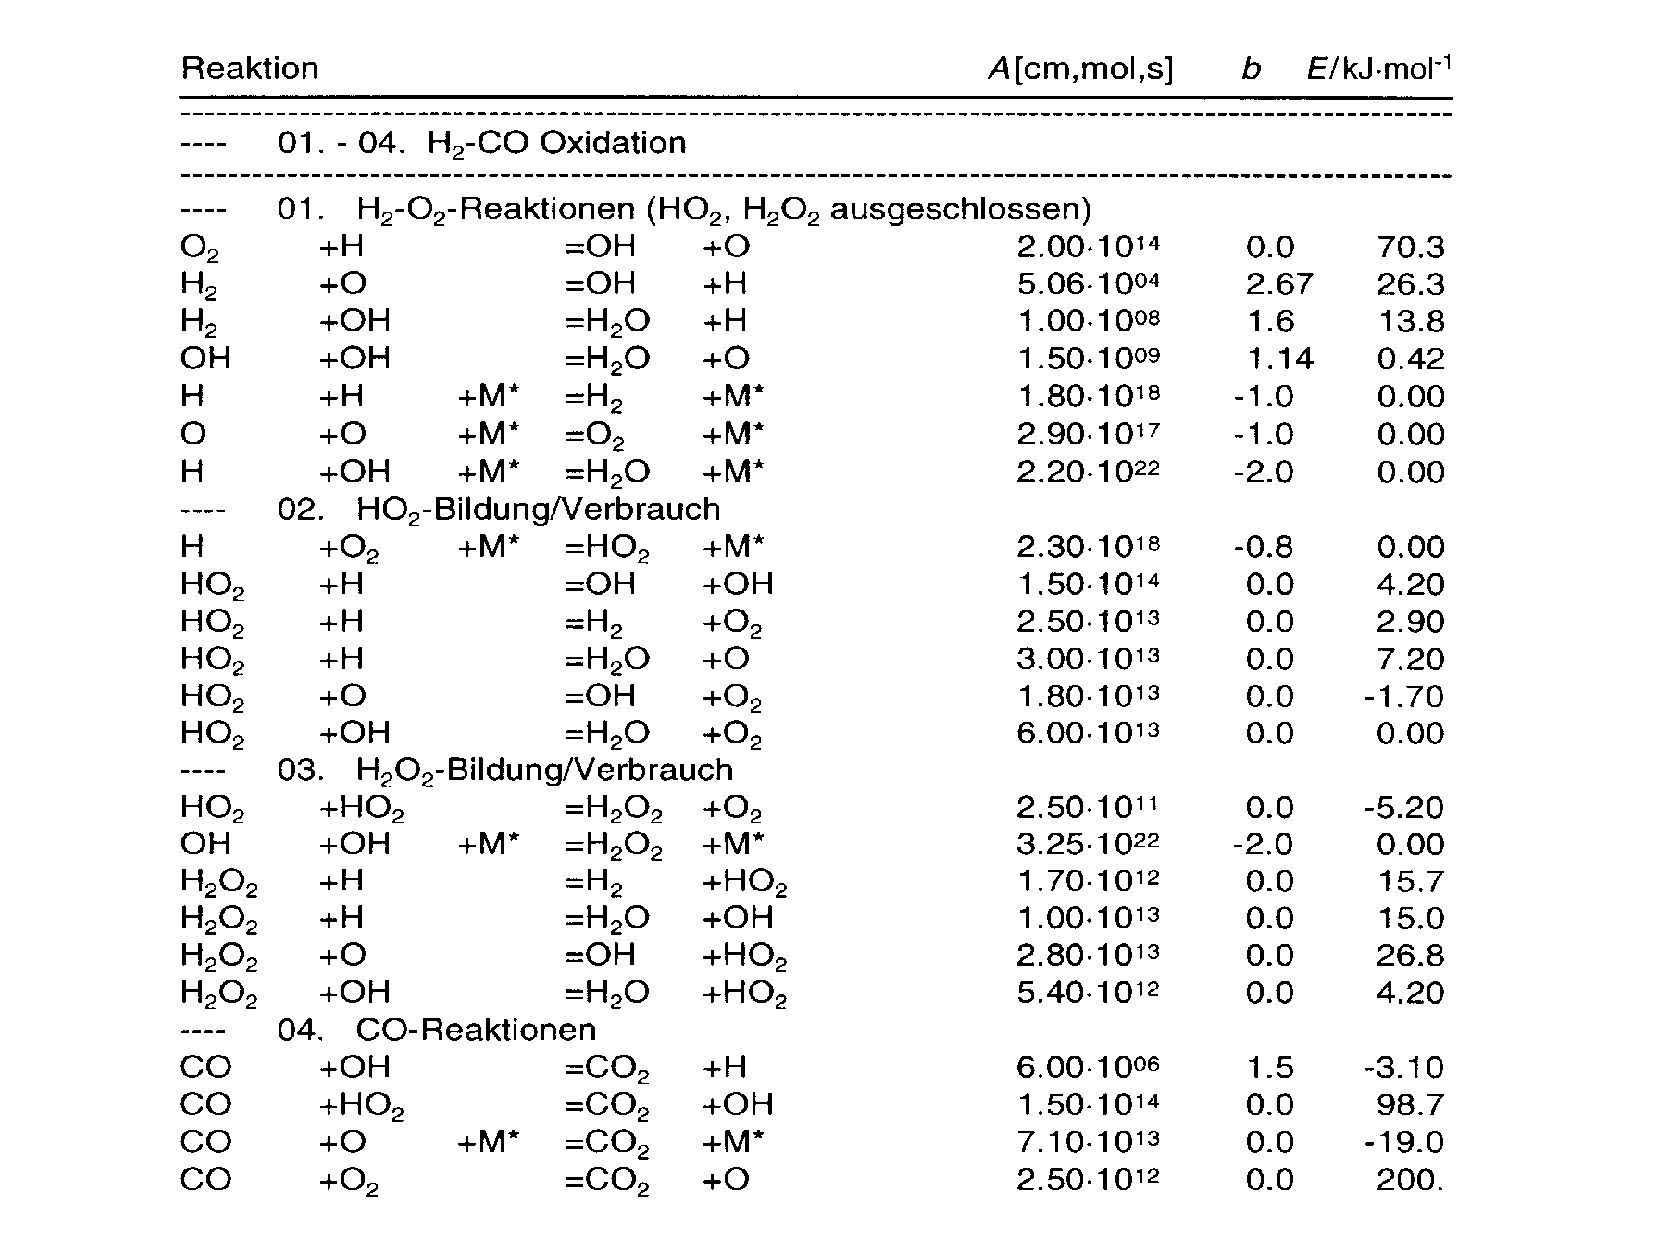
\includegraphics[width=1.3\columnwidth,clip]{./../Pics/ChemicalReactions_Reactions}}
      \end{figure}    \scriptsize\vspace{-.5cm}
       Elementary reactions in CH$_{4}$ / air combustion system. Extracted from Warnatz, Maas $\&$ Dibble (2006) $\lq$Combustion: Physical and Chemical Fundamentals, Modeling and Simulation, Experiments, Pollutant Formation'.
     \end{column}
     \begin{column}[l]{0.5\linewidth}%\scriptsize
        \begin{enumerate} \setcounter{enumi}{3}
           \item<1-> Multireaction progress:
               \visible<1->{\begin{displaymath}
                  d n_{i} = \sum\limits_{i}\nu_{i,j}d\varepsilon_{j}
               \end{displaymath}}
           \item<2-> Mole fractions of species:     
               \visible<2->{\begin{displaymath}
                  y_{i} = \frc{n_{i,0} + \sum\limits_{j}\nu_{i,j}\varepsilon_{j}} {n_{0} + \sum\limits_{j} \nu_{j}\varepsilon_{j}}
               \end{displaymath}}  
        \end{enumerate}
             \blue{where $j$ is the reaction index.}
     \end{column}
  \end{columns}
\end{frame}
\normalsize


%%%
%%% SECTION
%%%
\section{Reaction Equilibrium}
\subsection{General Remarks}

%%%
%%% Slide
%%%
%\scriptsize
\begin{frame}
  \frametitle{Reaction Equilibrium: General Remarks}
  \begin{columns}
     \begin{column}[l]{0.5\linewidth}\scriptsize
      \begin{figure}%
        \begin{center}
          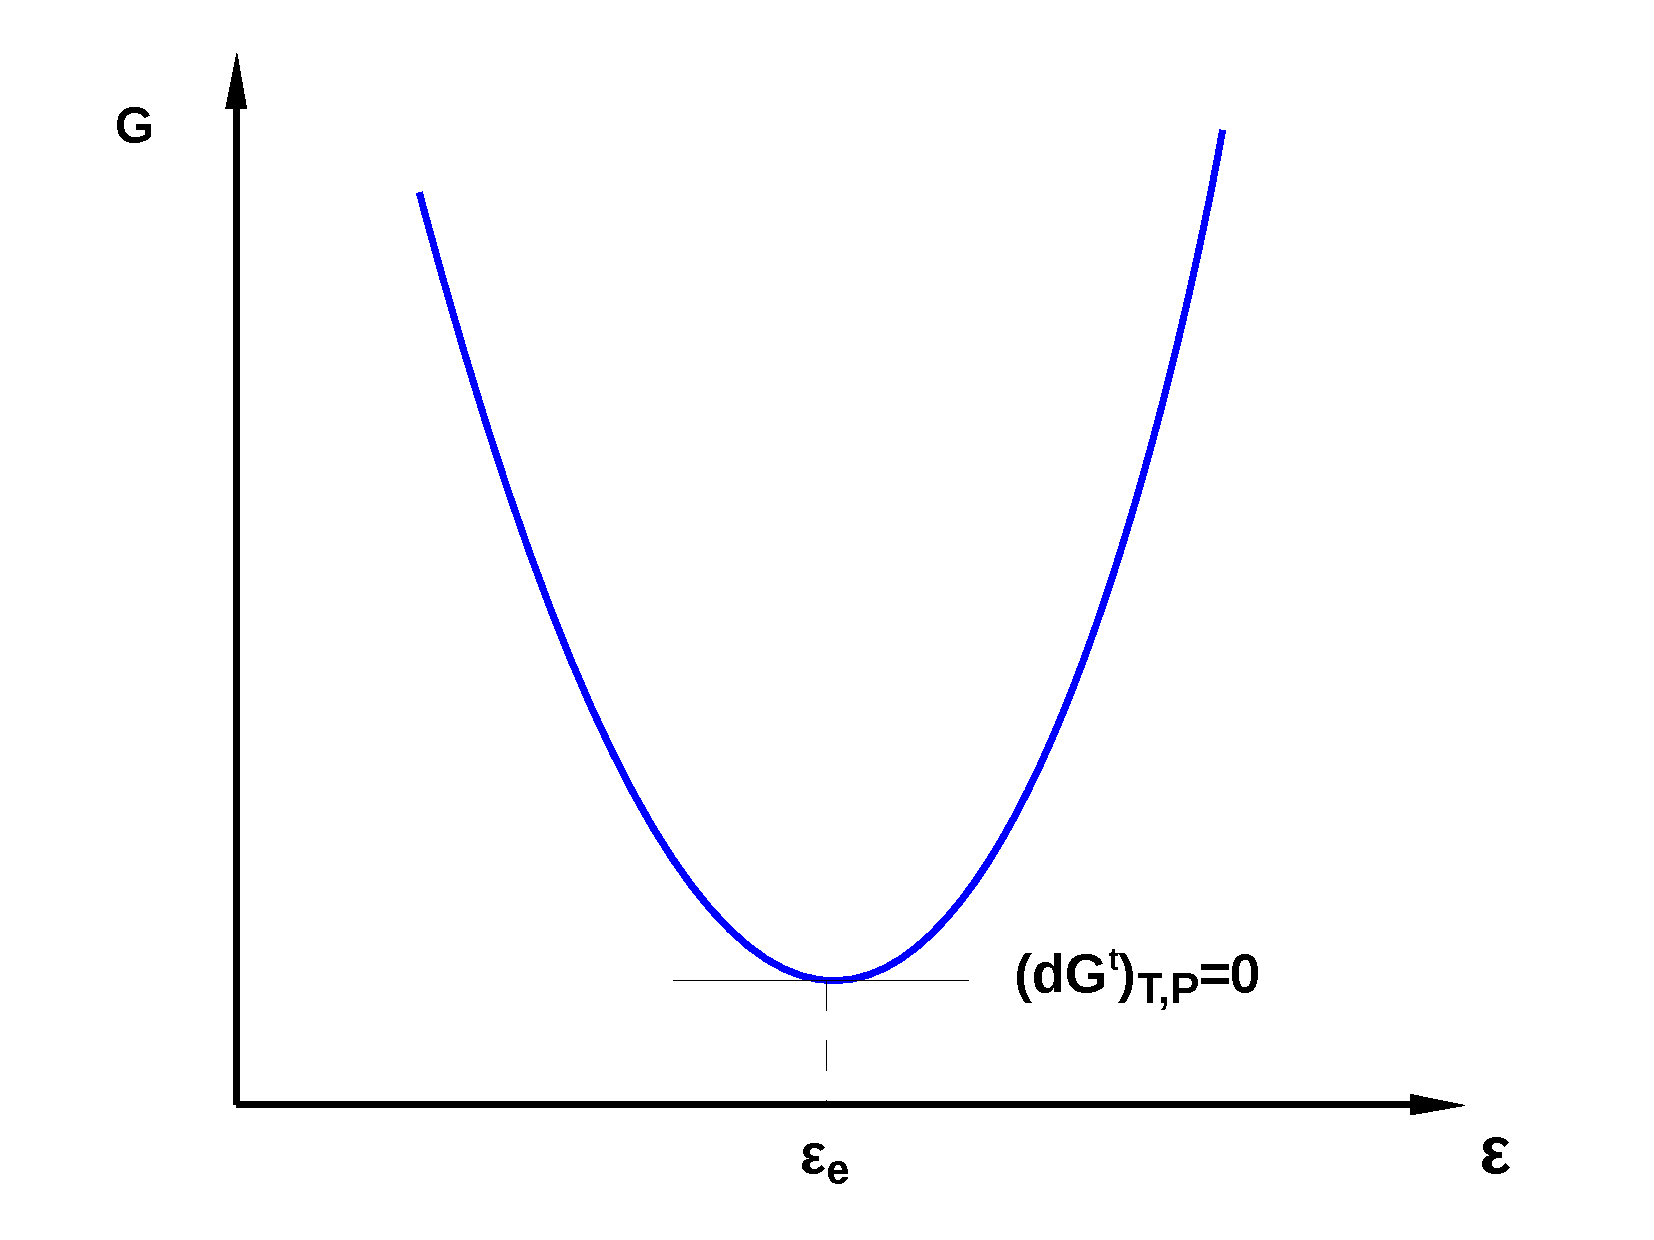
\includegraphics[width=1.05\columnwidth,clip]{./../Pics/ChemicalReactions_GxPlot}
        \end{center}
      \end{figure}
     \end{column}
     \begin{column}[l]{0.5\linewidth}%\scriptsize
        \begin{itemize} 
           \item<1-> From Module 04 we studied that the equilibrium criteria can be described as function of state properties (i.e., $G$, $S$, $U$ and $A$);
           \item<2-> In reactive systems, at constant $T$ and $P$, the equilibrium is reached when the \blue{total Gibbs energy} is \red{minimum}, i.e., 
               \visible<1->{\begin{displaymath}
                  \left(d G^{t}\right)_{T,P} = 0 
               \end{displaymath}}
        \end{itemize}
     \end{column}
  \end{columns}
\end{frame}
\normalsize


%%%
%%% SUBSECTION
%%%
\subsection{Equilibrium Constant}

%%%
%%% Slide
%%%
%\scriptsize
\begin{frame}
  \frametitle{Reaction Equilibrium: Equilibrium Constant}
      \begin{enumerate} 
         \item<1-> Criterion:
            \visible<1->{\begin{displaymath}
                \sum\limits_{i} \nu_{i}\mu_{i} = 0      
            \end{displaymath}}
         \item<2-> Equilibrium constant $K$:
               \visible<2->{\begin{displaymath}
                  \prod\limits_{i}\left(\frc{\overline{f}_{i}}{f_{i}^{0}}\right)^{\nu_{i}} = K =\exp\left(\frc{-\Delta G^{0}}{RT}\right)
               \end{displaymath}}
         \item<3-> Standard heat of reaction:
               \visible<2->{\begin{displaymath}
                   \Delta H^{0} = -RT^{2}\left[\frc{d \left(\frac{\Delta G^{0}}{RT}\right)}{d T }\right]
               \end{displaymath}}
      \end{enumerate}
\end{frame}
\normalsize


%%%
%%% Slide
%%%
%\scriptsize
\begin{frame}
  \frametitle{Reaction Equilibrium: Equilibrium Constant}
  \begin{columns}
     \begin{column}[l]{0.5\linewidth}\scriptsize
          \hspace{-3.1cm}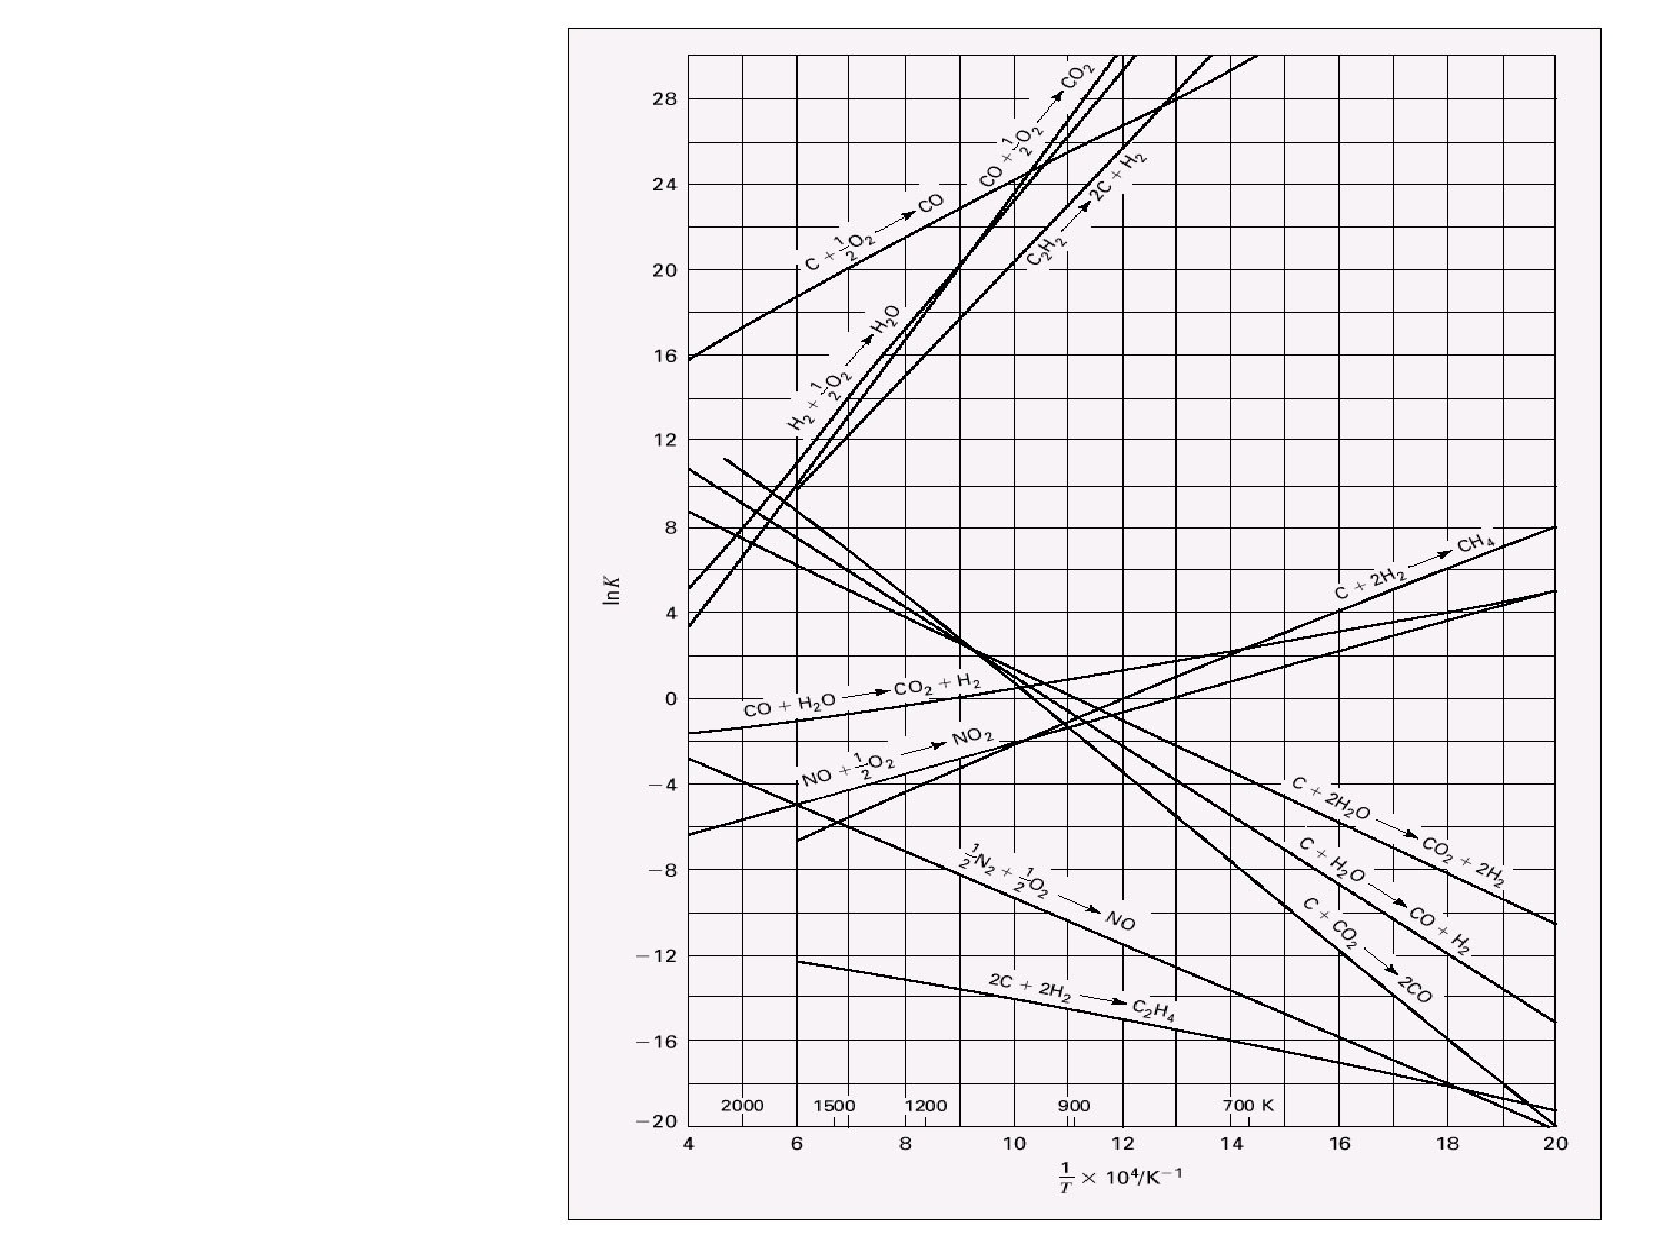
\includegraphics[width=1.5\columnwidth,clip]{./../Pics/ChemicalReactions_EquilConstPlot}
     \end{column}
     \begin{column}[l]{0.5\linewidth}%\scriptsize
        \begin{enumerate} \setcounter{enumi}{3}
            \item<1-> Temperature Effects:
                \begin{enumerate}%\scriptsize
                   \item<1-> On equilibrium constant:
                      \visible<1->{\begin{displaymath}\scriptsize
                         \frc{d\ln K}{d T} = \frc{\Delta H^{0}}{RT^{2}}
                      \end{displaymath}}
                   \item<2-> On standard heat of reaction:
                      \visible<2->{\begin{displaymath}\scriptsize
                         \Delta H^{0} = \Delta H_{0}^{0} + R\int\limits_{T_{0}}^{T} \frc{\Delta C_{p}}{R}dT
                      \end{displaymath}}
                \end{enumerate}
        \end{enumerate}
     \end{column}
  \end{columns}
\end{frame}
\normalsize


%%%
%%% Slide
%%%
%\scriptsize
\begin{frame}
  \frametitle{Reaction Equilibrium: Equilibrium Constant}
        \begin{enumerate} \setcounter{enumi}{4}
            \item<1-> Composition Effects:
                \begin{enumerate}%\scriptsize
                   \item<1-> In gas-phase reactions:
                      \visible<1->{\begin{displaymath}\scriptsize
                         \red{\prod\limits_{i}\left(y_{i}\phi_{i}\right)^{\nu_{i}} =K \left(\frc{P}{P^{0}}\right)^{-\nu},\hspace{1cm}\text{where } \nu=\sum\limits_{i}\nu_{i}}
                      \end{displaymath}}
                   \item<2-> In liquid phase reactions:
                      \visible<2->{\begin{displaymath}\scriptsize
                        \prod\limits_{i}\left(y_{i}\gamma_{i}\right)^{\nu_{i}} = K\exp\left[\frc{P^{0}-P}{RT}\sum\limits_{i}\left(\nu_{i}V_{i}\right)\right]^{-\nu},
                      \end{displaymath}}
                   \visible<2->{assuming that the liquid is incompressible with molar volume $V_{i}$.}
                   %\item<3-> Equilibrium conversion \blue{$\varepsilon_{e}$}
                \end{enumerate} 
        \end{enumerate}
\end{frame}
\normalsize

%%%
%%% SUBSECTION
%%%
\subsection{Phase Rule}

%%%
%%% Slide
%%%
%\scriptsize
\begin{frame}
  \frametitle{Reaction Equilibrium: Phase Rule}
     \begin{enumerate} %\setcounter{enumi}{4}
        \item<1-> Recall the Gibbs phase rule (Module 1) for \blue{non-reacting multiphase and multi-component systems}:
           \visible<1->{\begin{displaymath}
             \Psi = 2 + \mathcal{C} - \mathcal{P}
           \end{displaymath}
             where $\Psi$ is the number of \textcolor{blue}{degrees of freedom} for the system, \textcolor{blue}{2} refers to the independent variables ($T$ and $P$), \textcolor{blue}{$\mathcal{C}$} is the number of chemical species and \textcolor{blue}{$\mathcal{P}$} is the number of phases;}   
        \item<2->For a multiphase, multi-component systems with \red{$\mathcal{R}$ chemical reactions} take place: 
           \visible<1->{\begin{displaymath}
              \blue{\Psi = 2 + \mathcal{C} - \mathcal{P} - \mathcal{R}}
           \end{displaymath}}
     \end{enumerate}
\end{frame}
\normalsize

%%%
%%% SUBSECTION
%%%
\subsection{Multi-Reaction Equilibrium}

%%% Slide
%%%
%\scriptsize
\begin{frame}
  \frametitle{Multi-Reaction Equilibrium}
     \begin{enumerate} %\setcounter{enumi}{4}
        \item<1-> For a gas phase system (ideal gas):
            \visible<1->{\begin{displaymath}
               \red{\prod_{i}\left(y_{i}\right)^{\nu_{i,j}} = \left(\frc{P}{P^{0}}\right)^{-\nu_{i,j}}K_{j}}
            \end{displaymath}}
        \item<2-> Elemental material balance,
            \visible<2->{\begin{displaymath}
               \sum\limits_{i}n_{i}a_{ik} = A_{k}
            \end{displaymath}
            where \blue{$k$} and \blue{$i$} represent element and molecular species. \blue{$A$} is the total number of atomic masses and \blue{$a$} is the number of atoms.}
        \item<3-> Standard Gibbs energy change:
            \visible<3->{\begin{displaymath}  
               \Delta G^{0}_{f_{i}} + RT\ln\left(\frc{y_{i}\overline{\phi}_{i}P}{P^{0}}\right) + \sum\limits_{k}\lambda_{k}a_{ik} = 0\;\;\;i=1,2,\cdots,\mathcal{C}
               \end{displaymath}} 
     \end{enumerate}
\end{frame}
\normalsize

\section{Summary}

%%%
%%% Slide
%%%
%\scriptsize
\begin{frame}
 \frametitle{Summary}
   After this Module, you should be able to:
   \begin{enumerate}[(i)]
     \item Identify and make use of chemical notation for reacting thermodynamic systems;
     \item Identify thermodynamic criteria for chemical equilibrium;
     \item Make use of equilibrium constant definition and its dependence on system parameters;
     \item Apply phase rule for reacting systems.
   \end{enumerate}
\end{frame}


\end{document}
 
